\section{Actividad 2: Curva Característica de un Diodo}

 \subsection{Objetivo:}
 Realizar mediciones de corrientes y tensiones de los diodos rectificadores tanto
de Silicio como el de Germanio. Identificar principalmente el codo de conmutación entre el
estado de bloqueo a conducción y comparar estos datos con las especificaciones del
fabricante.


\subsection{Simulacion de Polarización en Directa:}

Primero implementamos el siguiente circuido en el simulador LTSpice:

\begin{figure}[ht!]
    \centering
    \begin{circuitikz}[american, scale=1.3, transform shape]
        \draw
        (0,0) to[battery, l=$V_1$] (0,3)
        (0,3) to[R, l=$R_1$] (2.8,3)
        (2.8,3) to[D, l_=$D_1$] (2.8,0)
        (2.8,0) -- (0,0)
        ;
        % Add ground at (0,0)
        \draw (0,0) node[ground]{};
    \end{circuitikz}
    \caption{}
\end{figure}

El circuito completo con sus respectivos valores es el siguiente:\\

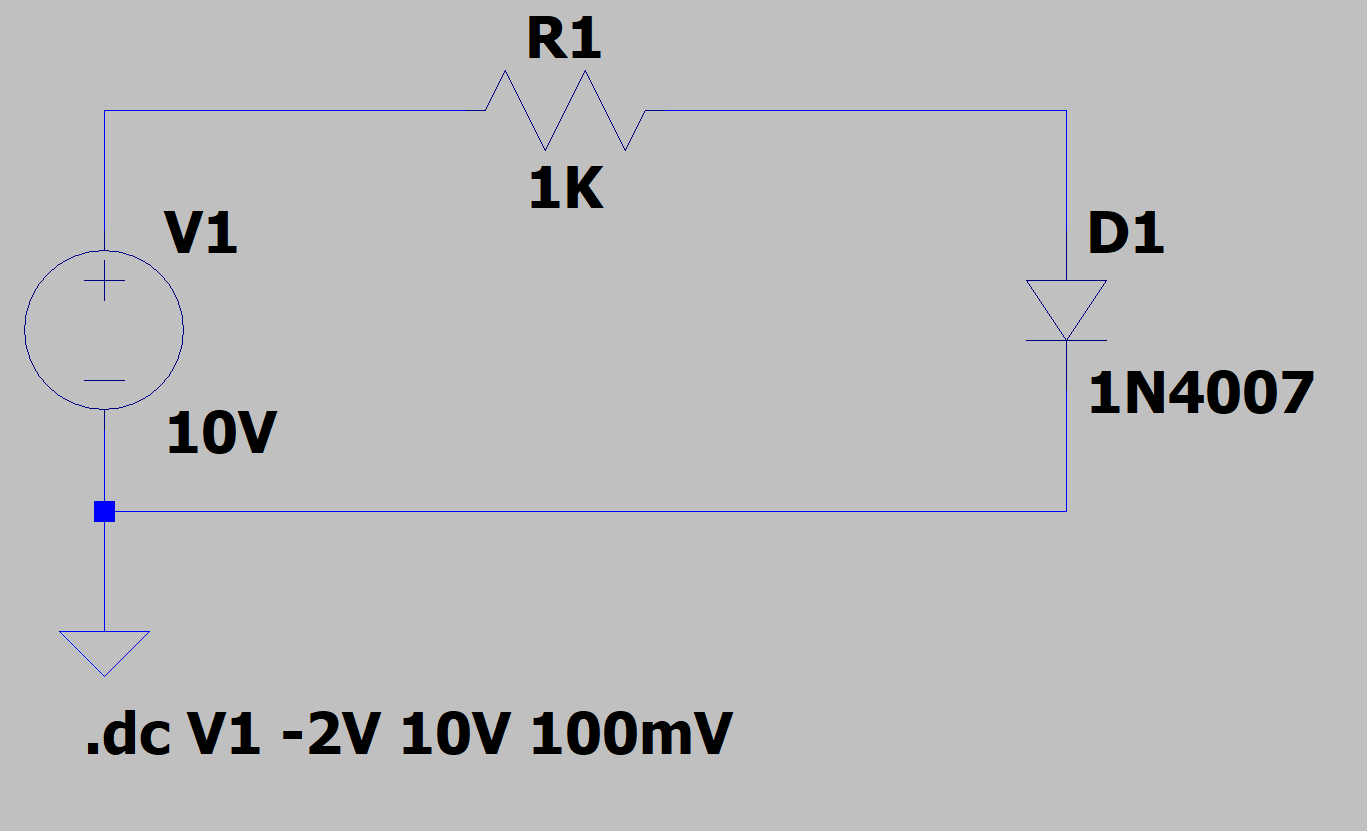
\includegraphics[width=9.3cm]{imagenes/Circuito1.png}\\

Luego de simular el circuito, obtenemos la siguiente curva característica:

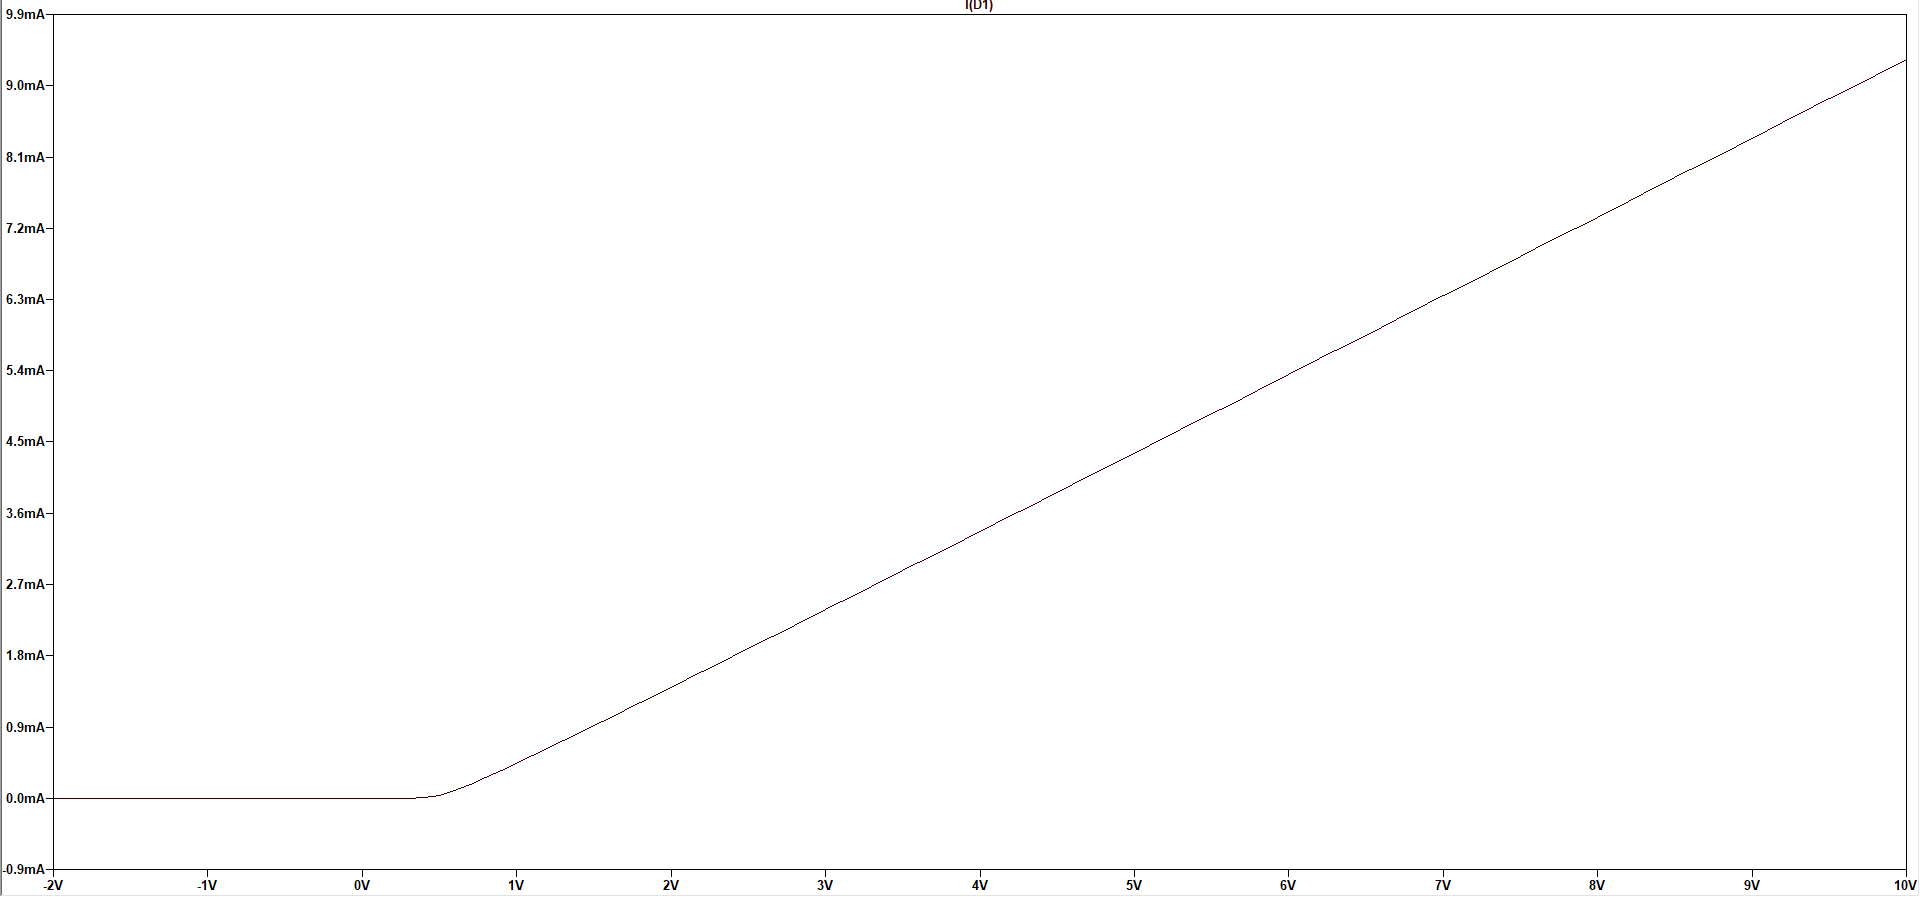
\includegraphics[width=9cm]{imagenes/simulacion11.png}\\

Ahora repetimos el proceso para el diodo de germanio, obteniendo el siguiente circuito:

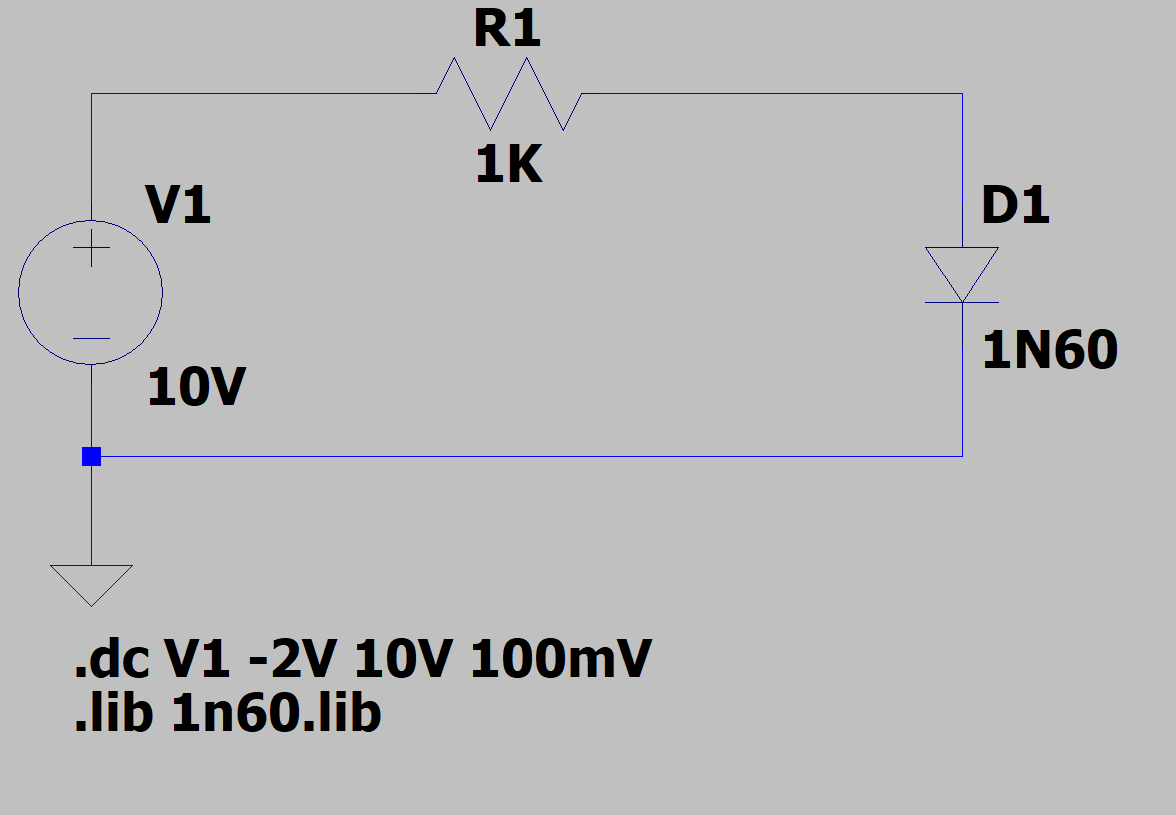
\includegraphics[width=8cm]{imagenes/Circuito2.png}\\

Y la curva característica:

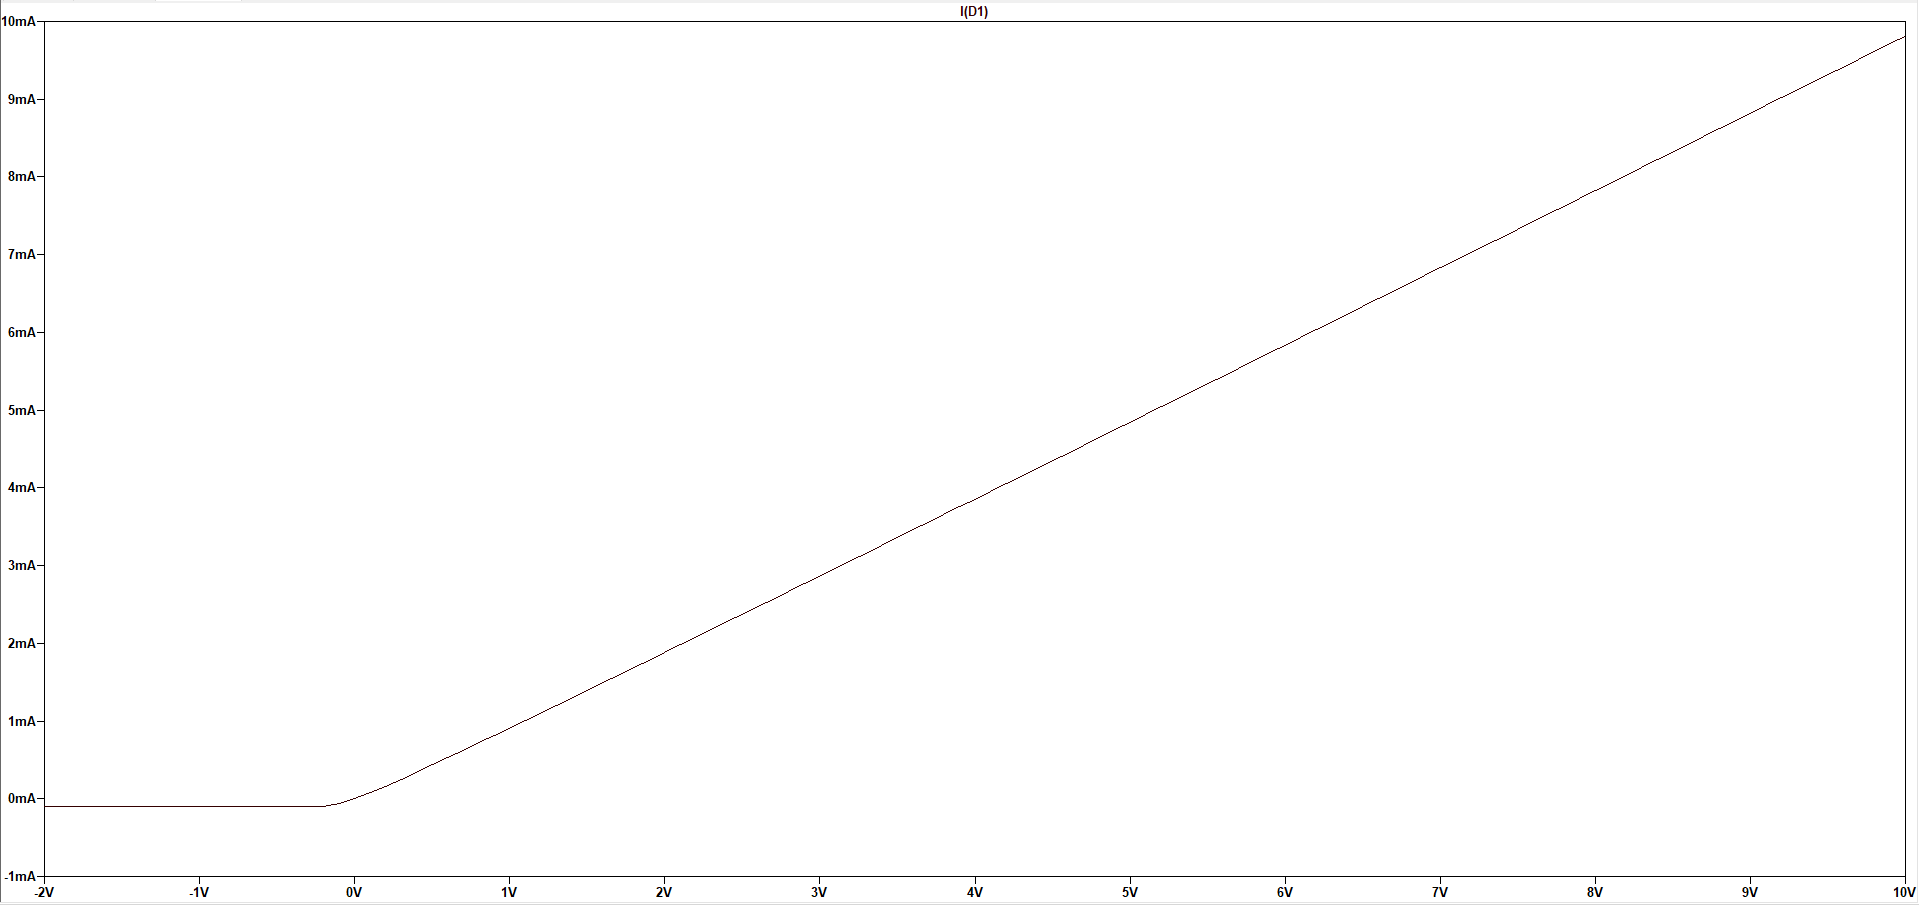
\includegraphics[width=8.2cm]{imagenes/simulacion2.png}\\

\subsection{Conslusiones de Polarizacion en Directa:}

(AÑADIR CONCLUSIONES)

\vspace{1cm}

\subsection{Simulacion de Polarización en Inversa:}

Para la polarizacion en inversa debemos conocer el voltaje de ruptura del diodo, en el caso del 1N4007 es de 1000V y el del 1N60 es de 40V. Por lo que configuramos el simulador para obtener valores que superen esos:

\vspace{1cm}

\paragraph{Diodo de Silicio 1N4007:}

Circuito:
\vspace{0.5cm}

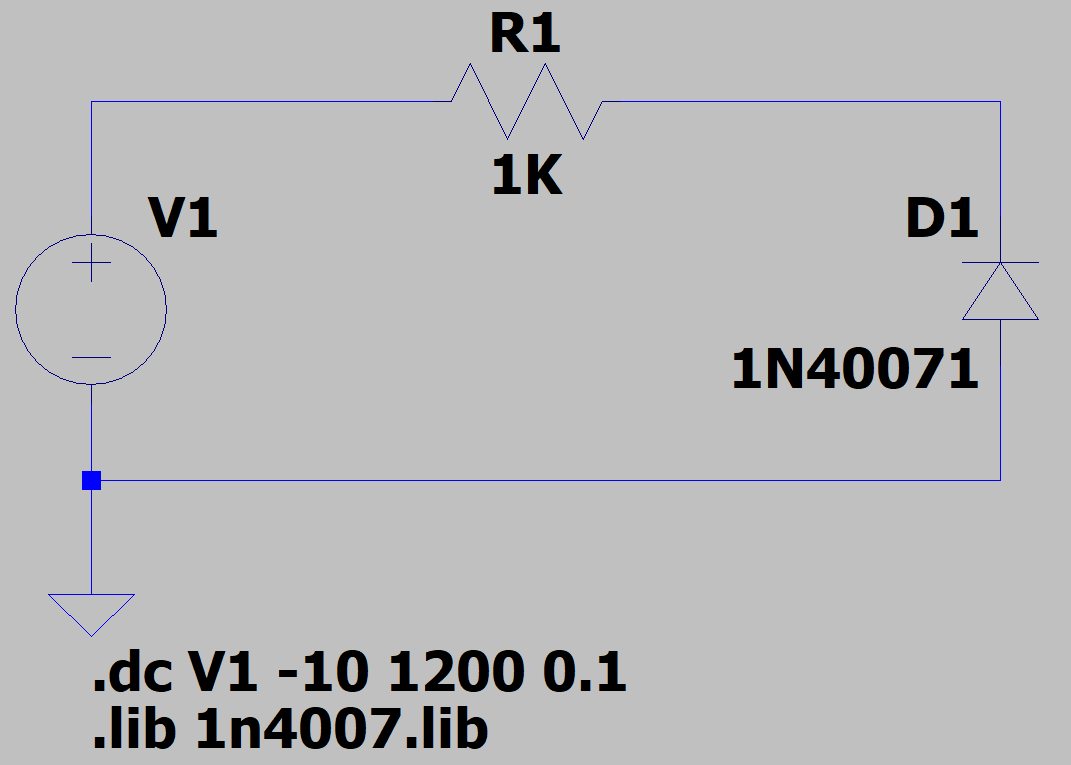
\includegraphics[width=8cm]{imagenes/Circuito3.PNG}

\vspace{0.5cm}

Simulación:

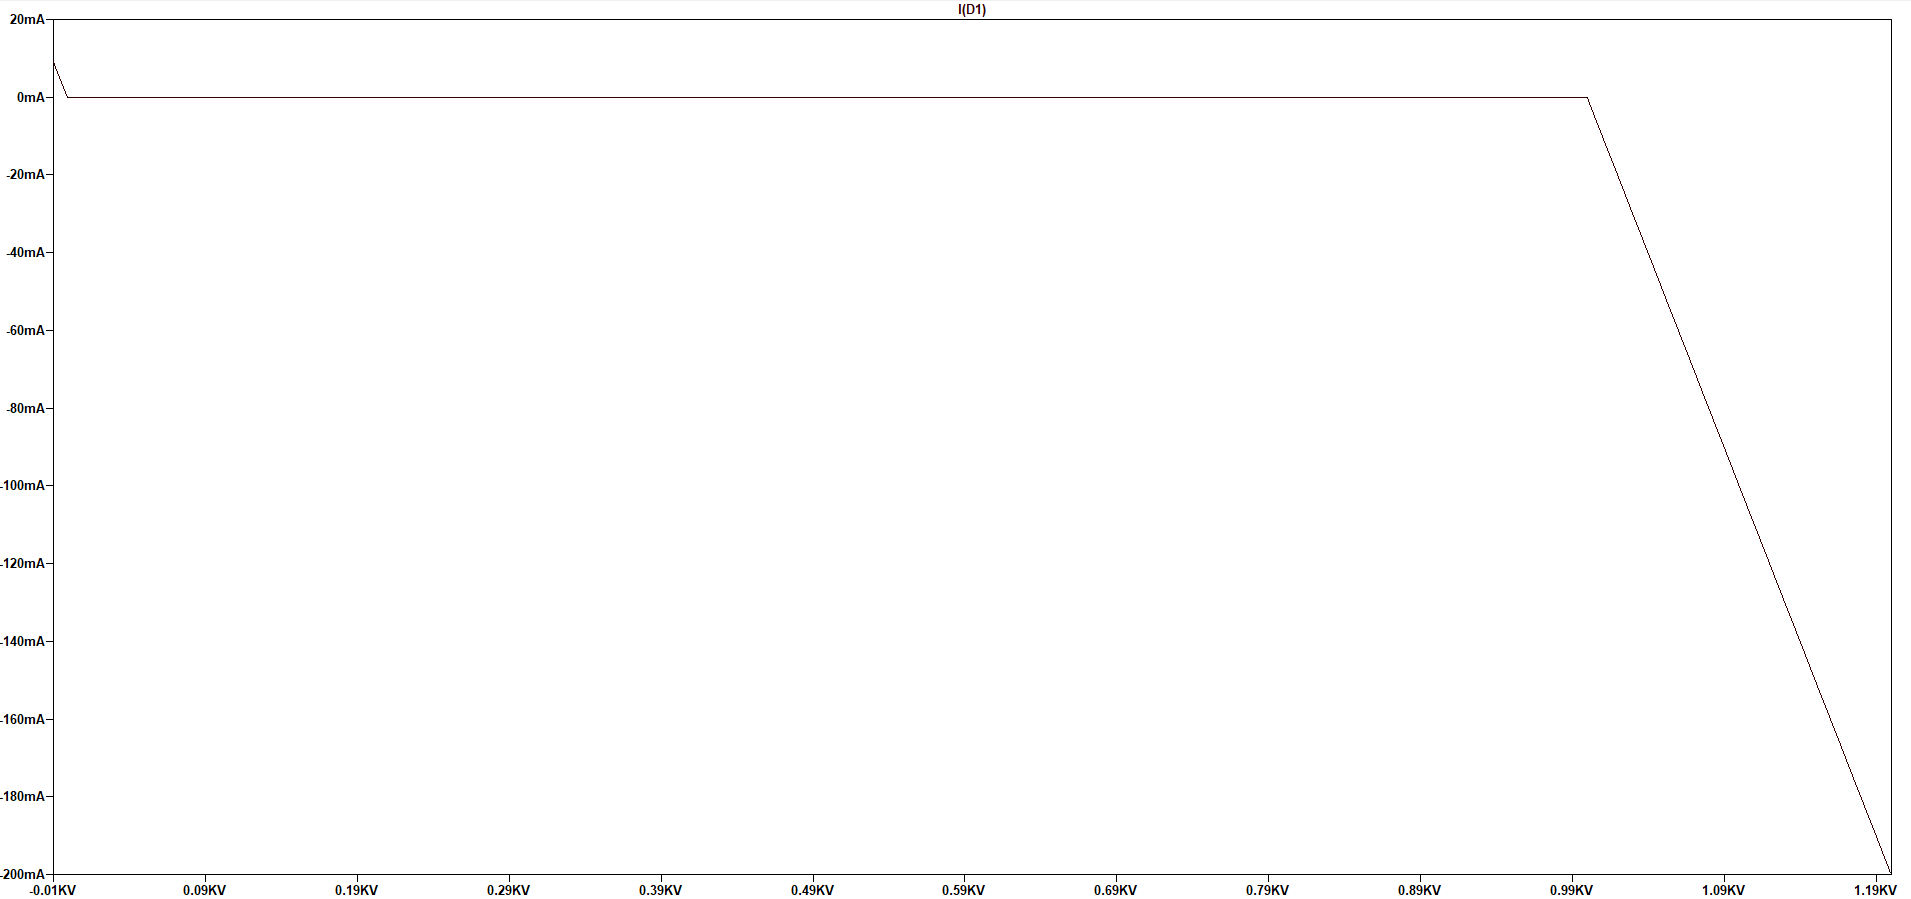
\includegraphics[width=8.2cm]{imagenes/simulacion3.png}\\

\paragraph{Diodo de Germanio 1N60:}

Circuito:

\vspace{0.5cm}

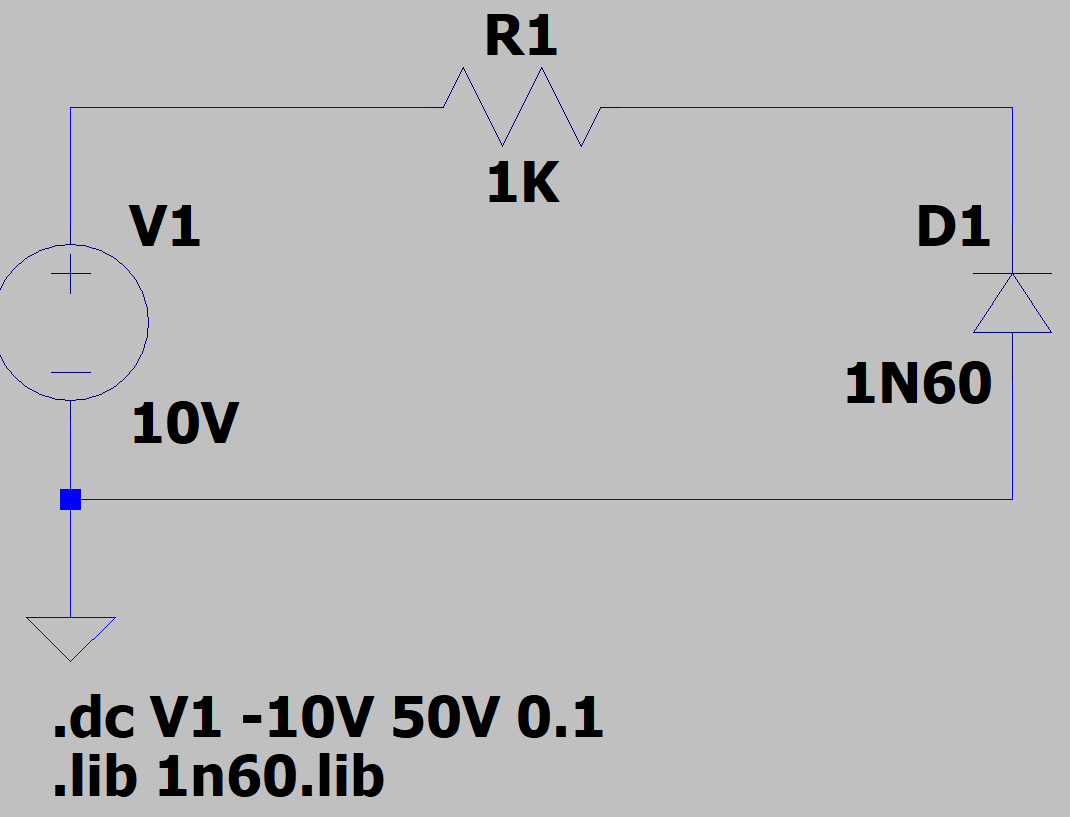
\includegraphics[width=8cm]{imagenes/Circuito4.png}\\

\vspace{0.5cm}

Simulación:

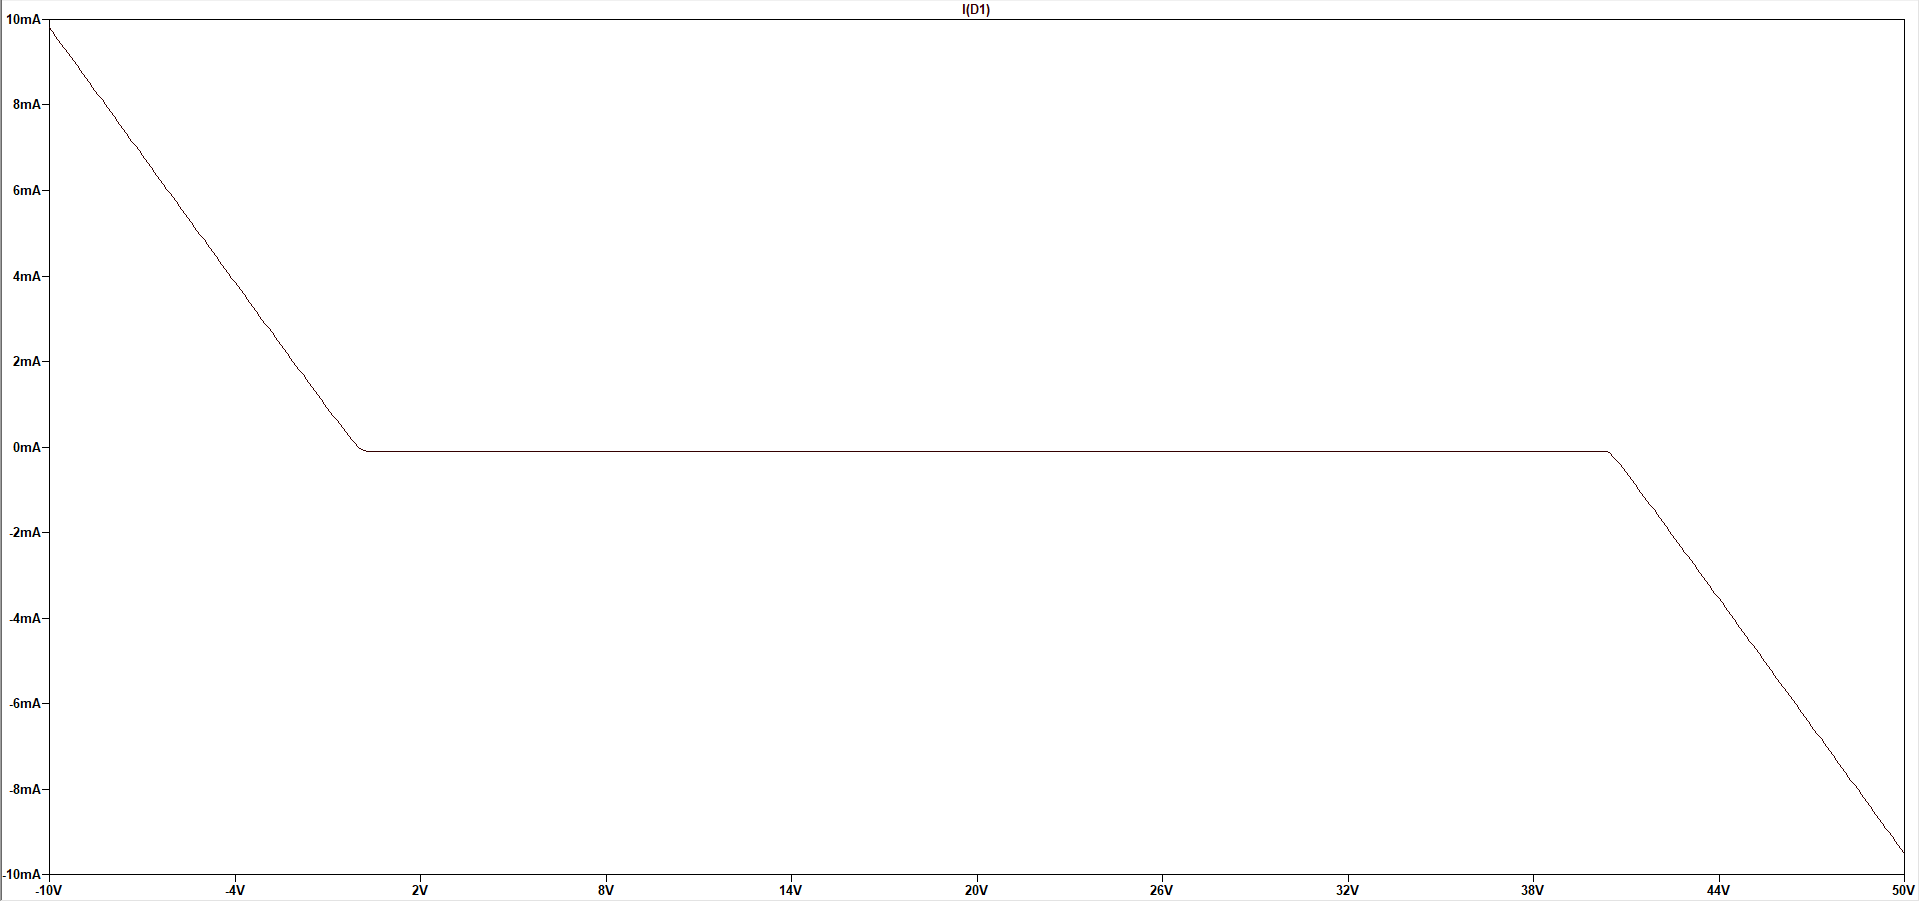
\includegraphics[width=8.2cm]{imagenes/simulacion4.png}\\

\subsection{Conclusiones de Polarizacion en Inversa:}
(AÑADIR CONCLUSIONES)


\subsection{Laboratorio:}
 